\documentclass[a4paper,abstract=on,twoside]{scrreprt}

\usepackage[todo]{../../common/naps62}

\hypersetup{pdfauthor={Miguel Branco Palhas}}
\hypersetup{pdftitle={Pre-Thesis: An Evaluation of the GAMA Framework for Heterogeneous Platforms: The Progressive Photon Mapping Algorithm}}

\bibliography{../../common/bib/gama,../../common/bib/gpu,../../common/bib/photon_mapping}

% reduce chapter margins
\renewcommand{\chapterheadstartvskip}{\vspace*{-1.6\baselineskip}}

\begin{document}
\pdfbookmark{Cover}{cover}
\pagenumbering{roman}
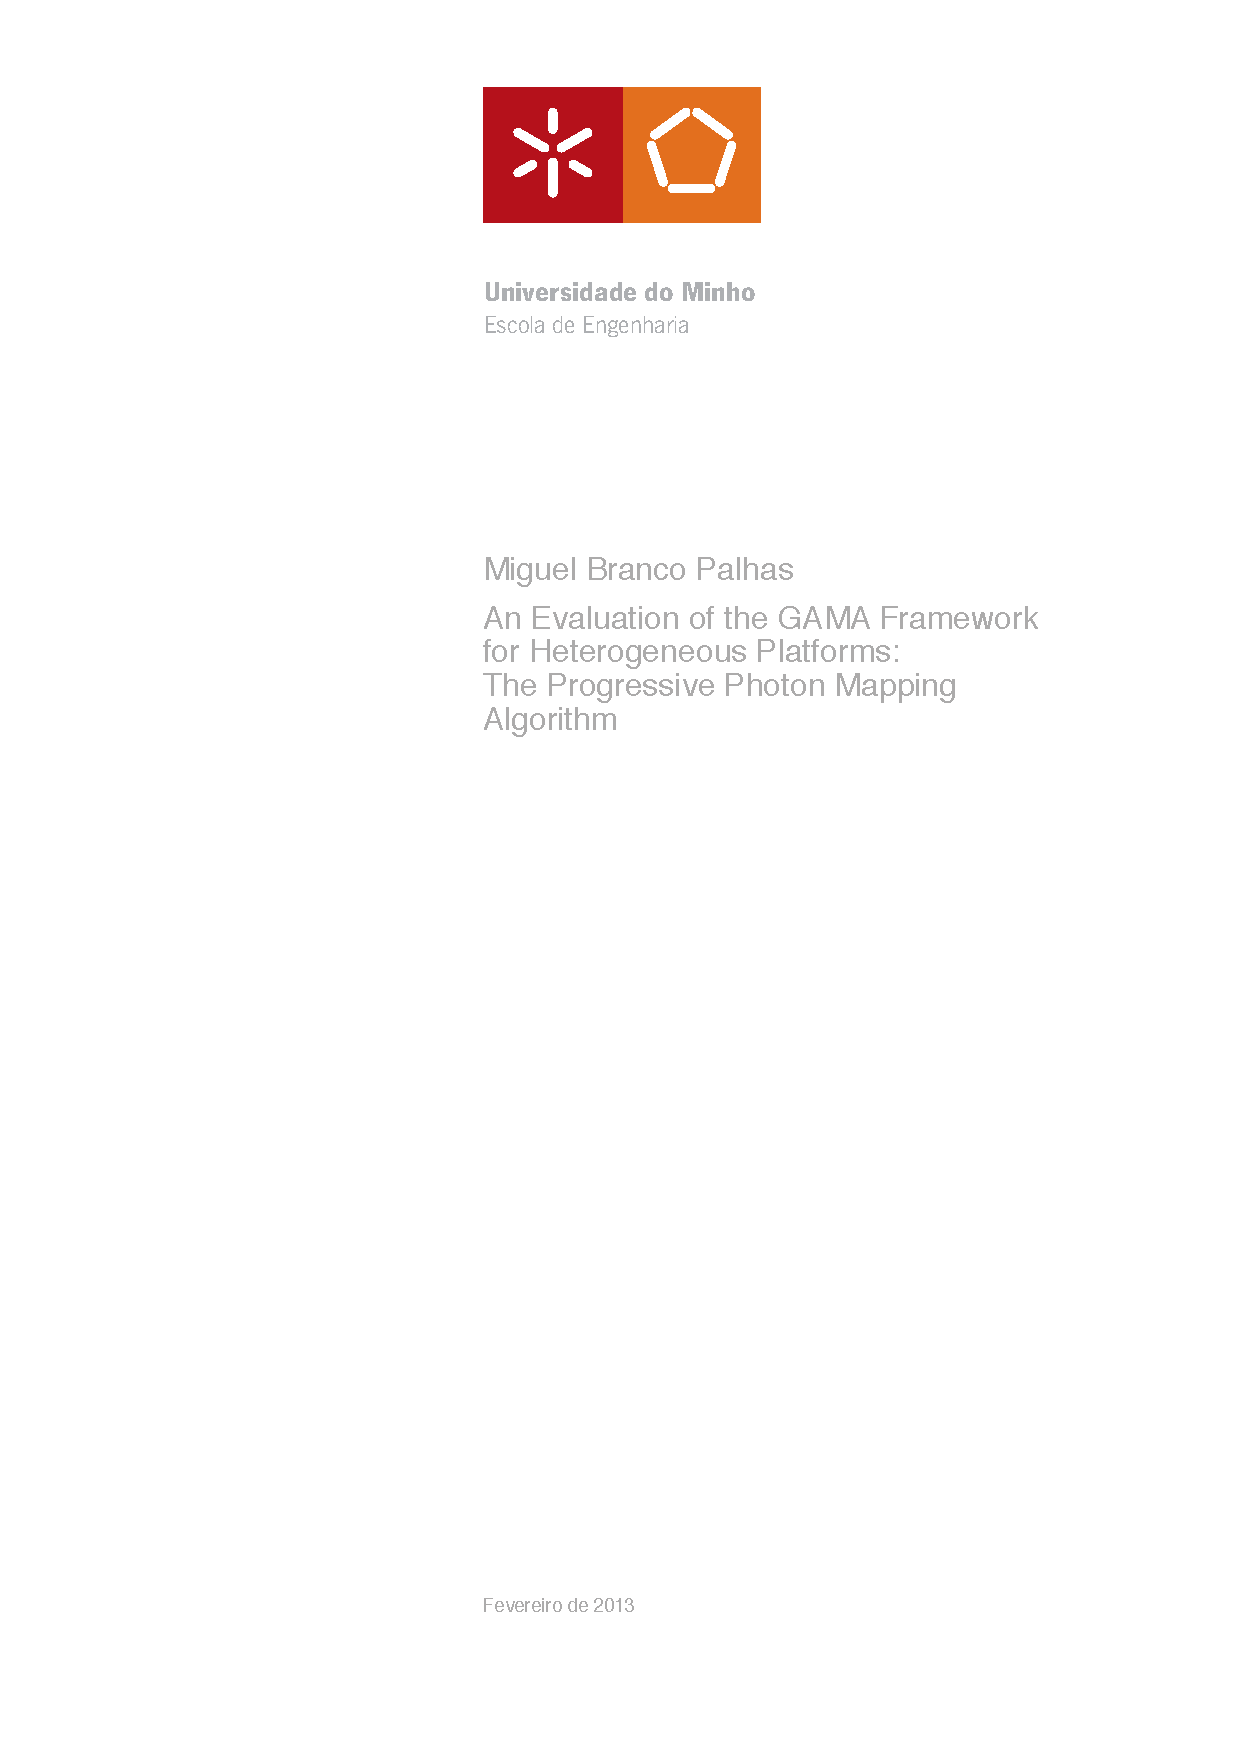
\includepdf[pages=-]{misc/cover-mei}

\pagestyle{fancy}
\renewcommand{\headrulewidth}{0.4pt}
\fancyhead[LO,RE]{}
\fancyhead[LE]{\slshape \leftmark}
\fancyhead[RO]{\slshape \rightmark}
\fancyfoot[RO,LE]{\thepage}%
\fancyfoot[C]{}

\fancypagestyle{plain}{%
  \renewcommand{\headrulewidth}{0.0pt}
  \fancyhead{}
  \fancyfoot[C]{}
  \fancyfoot[RO,LE]{\thepage}
}


%
% include all tex/ chapter files
%
\bash[stdoutFile=/dev/null,stderrFile=/dev/null,exitCodeFile=/dev/null,scriptFile=bash.out]
ls tex/ | egrep ^[^_] | sed "s/\([^.]*\)\.tex/\\\\subfile{tex\/\1}/" > tex/_inputs.tex
\END
\subfile{tex/000_abstract}
\subfile{tex/001_next}



%\bibliographystyle{../../common/IEEE}
%\nocite{*}
\newpage % force the bookmark to go to the new page
\pdfbookmark{References}{references}
\printbibliography

\end{document}
